% experimental.tex
\documentclass[main.tex]{subfiles}
\begin{document}
\chapter{Experimental methods} \label{ch:exp}
\section{Material} \label{sec:material}

The first step of the experimental work involved development of a custom thermoplastic filament for the FFF process. The reasoning behind this decision was two-fold. First, the use of an off the shelf, commercial thermoplastic filament generally does not guarantee that two different spools were produced under the same processing conditions \textemdash or even using the same parent material. Secondly, the results from Koch \emph{et al.} \cite{Koch2017} suggest that fluctuations in the filament diameter can produce a significant impact in the mechanical properties of FFF parts due to improper volumetric output at the nozzle during the printing process. 

The resin chosen was Cycolac\texttrademark MG94, produced by SABIC. This is an Acrylonitrile Butadiene Styrene (ABS) resin traditionally used for injection molding thin walled parts, as well as extrusion of FFF filament. With a reported Melt Flow Index of 11.7 g/10 min, it is an ideal resin for both the FFF and extrusion processes. The MG94 was extruded in a setup that consisted of a single screw extruder (Extrudex EDN 45X30D, Germany) with 45 mm screw diameter and L/D ratio of 30D. The hot melt was extruded at 205 $^\circ$C through a circular die with a 5.8 mm diameter, and then guided through a pre-skinner into a vacuum-assisted, heated water bath (Conair, USA) to cool the extrudate whilst minimizing void formation. The solidified filament was then passed through a 3-axis laser micrometer (LaserLinc, USA) and a belt puller (Conair, USA) configured in a control loop. The dimensions of the filament were adjusted by automatically changing the speed of the puller to keep the extrudate within specification. The desired filament dimensions were a diameter of 2.85 mm with a tolerance of $\pm$ 0.02 mm. Finally, the filament is wound onto big spools. A schematic of the extrusion setup can be seen in Figure \ref{fig:extrLine}.

\begin{figure}[h]
	\center
	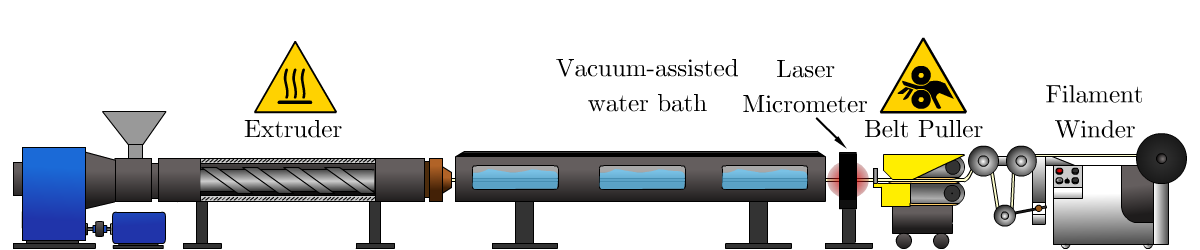
\includegraphics[width=\linewidth]{Extrusion_line}
	\caption{Extrusion line setup} \label{fig:extrLine}
\end{figure}

% Nomenclature introduced in this chapter:
\nomenclature[A]{ABS}{Acrylonitrile Butadiene Styrene}% 

% Symbols introduced in this chapter:
%\nomenclature[S]{$X_t$}{Tensile strength in the 1-1 direction \nomunit{$MPa$}}
\end{document}